% ============================================================
% Final Project Presentation
% Project 07: Document-Level OCR with Post-OCR Correction
% Course: CSC15012 - Applications of NLP in Industry
% Student: Le Dinh Minh Quan - 23127460 - 23CNTThuc
% Template based on Madrid + seahorse (Overleaf Beamer)
% ============================================================

\documentclass[10pt,aspectratio=169]{beamer}

\mode<presentation>
{
  \usetheme{Madrid}
  \usecolortheme{seahorse}
  \usefonttheme{default}
  \setbeamertemplate{navigation symbols}{}
  \setbeamertemplate{caption}[numbered]
  \setbeamertemplate{footline}[frame number]
}

% ---- Packages ----
\usepackage[english]{babel}
\usepackage[utf8]{inputenc}
\usepackage{amsmath}
\usepackage{graphicx}
\usepackage{booktabs}
\usepackage{xcolor}
\usepackage{hyperref}
\usepackage{xurl}
\usepackage{tikz}
\usepackage{pgfplots}
\pgfplotsset{compat=1.18}
\usetikzlibrary{shapes.geometric, arrows.meta, positioning, fit, backgrounds, shadows}
\usepackage{listings}
\lstset{
  basicstyle=\ttfamily\scriptsize,
  breaklines=true,
  frame=single,
  backgroundcolor=\color{gray!10},
  keywordstyle=\color{blue},
  commentstyle=\color{green!60!black},
  stringstyle=\color{red!70!black},
  showstringspaces=false,
  tabsize=2
}

% ---- HCMUS LOGO ----
% Upload logo_hcmus.png to Overleaf to display the logo (top-right of every slide).
% If the file is missing, no logo is shown (no error).
\IfFileExists{logo_hcmus.png}{\logo{\includegraphics[height=0.7cm]{logo_hcmus.png}}}{}

% ---- TITLE METADATA ----
\title[Project 07: Document-Level OCR]{Project 07: Document-Level OCR with Post-OCR Correction}
\subtitle{A Layout-Aware OCR Pipeline with a Trainable ByT5 Corrector and an Agentic Orchestrator}
\author[Le Dinh Minh Quan]{Le Dinh Minh Quan \\ \small ID: 23127460 -- Class: 23CNTThuc}
\institute[HCMUS]{Vietnam National University Ho Chi Minh City \\ University of Science -- Faculty of Information Technology \\ \small Course: CSC15012 -- Applications of NLP in Industry}
\date{2026}

\begin{document}

% ============================================================
% SLIDE 1: TITLE
% ============================================================
\begin{frame}
  \titlepage
\end{frame}

% ============================================================
% SLIDE 2: OUTLINE
% ============================================================
\begin{frame}{Outline}
\begin{columns}[T]
\begin{column}{0.5\textwidth}
\begin{enumerate}
  \item Business Problem \& Motivation
  \item Solution \& Success Metrics
  \item System Architecture
  \item Repository \& Tech Stack
  \item Data Overview
  \item Training / Autopilot Workflow
  \item Model Selection (Why ByT5)
\end{enumerate}
\end{column}
\begin{column}{0.5\textwidth}
\begin{enumerate}
  \setcounter{enumi}{7}
  \item Evaluation Results \& Safety Gate
  \item Agentic AI Component (D1--D4)
  \item Agent Example Interaction
  \item Deployment
  \item Ethics, Privacy \& Fairness
  \item Monitoring \& Continual Learning
  \item Key Takeaways \& Future Work
  \item Resources \& Thank You
\end{enumerate}
\end{column}
\end{columns}
\end{frame}

% ============================================================
% SLIDE 3: BUSINESS PROBLEM & MOTIVATION
% ============================================================
\begin{frame}{1. Business Problem \& Motivation}
\begin{block}{Context}
A flat OCR pass gives an \textbf{unordered, error-riddled} text dump: wrong reading order on multi-column pages, no block typing, and char-level garble (\texttt{rn$\rightarrow$m}, \texttt{0$\leftrightarrow$O}, \texttt{1$\leftrightarrow$l}, merged/split words). Clean structured text is the upstream feed for search, RAG, analytics, and compliance.
\end{block}

\begin{columns}[T]
\begin{column}{0.5\textwidth}
\textbf{Three product levers}
\begin{itemize}
  \item \textbf{Accuracy} -- a trained corrector lowers errors
  \item \textbf{Structure} -- Markdown/JSON, typed + ordered blocks
  \item \textbf{Engine-agnostic uplift} -- improves \emph{any} OCR backend, compounds with cheap CPU OCR
\end{itemize}
\end{column}
\begin{column}{0.5\textwidth}
\textbf{Stakeholders}
\begin{itemize}
  \item Archivists \& libraries
  \item Businesses digitizing records
  \item Accessibility users (screen readers)
  \item Developers \& researchers (REST API)
\end{itemize}
\end{column}
\end{columns}
\end{frame}

% ============================================================
% SLIDE 4: SOLUTION + SUCCESS METRICS
% ============================================================
\begin{frame}{2. Solution \& Success Metrics}
\begin{block}{Solution}
End-to-end \textbf{Document-Level OCR}: OCR front-end + layout/reading-order (structure) + a \textbf{trainable ByT5 post-OCR corrector} (accuracy) + a deterministic \textbf{agent} + REST API + Colab autopilot.
\end{block}

\begin{table}[h]
\centering\small
\begin{tabular}{lll}
\toprule
\textbf{Type} & \textbf{Metric} & \textbf{Target} \\
\midrule
Business  & Manual-review reduction (\% pages auto-accepted) & Maximize \\
Business  & Structure fidelity (\% blocks typed + ordered) & High \\
Technical & \textbf{CER reduction} vs.\ identity floor 0.088 & Clearly $>$0 \\
Technical & \textbf{Safety gate}: \% degraded $\ll$ \% improved & Hard go/no-go \\
Technical & Latency, born-digital page (D2 skip) & $\sim$200\,ms \\
\bottomrule
\end{tabular}
\end{table}

\textbf{Headline KPI} = CER/WER \emph{reduction} vs.\ the raw-OCR identity baseline, gated so the corrector is a net help \emph{per example}, not just on average.
\end{frame}

% ============================================================
% SLIDE 5: SYSTEM ARCHITECTURE (TikZ)
% ============================================================
\begin{frame}{3. System Architecture}
\centering
\resizebox{0.92\linewidth}{!}{%
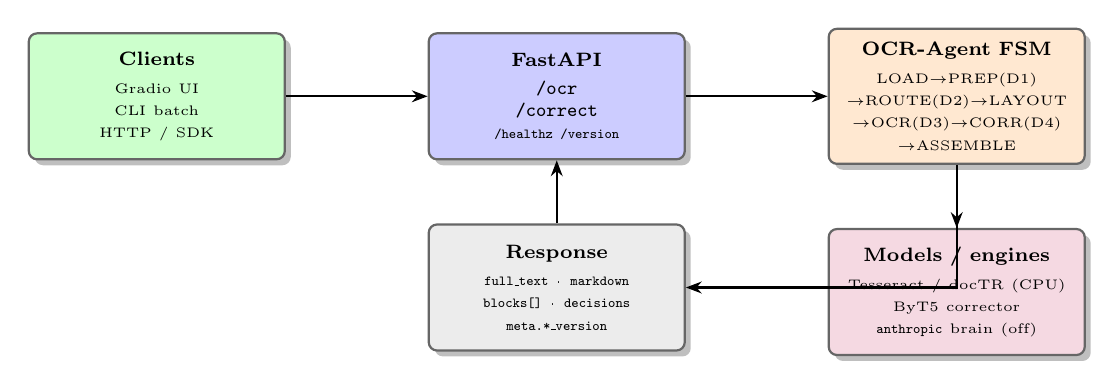
\begin{tikzpicture}[
  node distance=0.8cm and 1.8cm,
  box/.style={rectangle, draw=black!60, rounded corners=3pt, thick,
             text width=2.9cm, minimum height=1.6cm, align=center,
             inner sep=5pt, font=\scriptsize, drop shadow},
  clientbox/.style={box, fill=green!20},
  apibox/.style={box, fill=blue!20},
  agentbox/.style={box, fill=orange!18},
  modelbox/.style={box, fill=purple!15},
  arrow/.style={-{Stealth[length=2mm]}, thick}
]
\node[clientbox] (client) {%
  \textbf{Clients}\\[2pt]
  {\tiny Gradio UI}\\ {\tiny CLI batch}\\ {\tiny HTTP / SDK}
};
\node[apibox, right=of client] (api) {%
  \textbf{FastAPI}\\[2pt]
  \texttt{/ocr}\\ \texttt{/correct}\\
  {\tiny \texttt{/healthz} \texttt{/version}}
};
\node[agentbox, right=of api] (agent) {%
  \textbf{OCR-Agent FSM}\\[2pt]
  {\tiny LOAD$\rightarrow$PREP(D1)}\\
  {\tiny $\rightarrow$ROUTE(D2)$\rightarrow$LAYOUT}\\
  {\tiny $\rightarrow$OCR(D3)$\rightarrow$CORR(D4)}\\
  {\tiny $\rightarrow$ASSEMBLE}
};
\node[modelbox, below=0.8cm of agent] (models) {%
  \textbf{Models / engines}\\[2pt]
  {\tiny Tesseract / docTR (CPU)}\\
  {\tiny ByT5 corrector}\\
  {\tiny \texttt{anthropic} brain (off)}
};
\node[box, fill=gray!15, below=0.8cm of api, text width=2.9cm] (out) {%
  \textbf{Response}\\[2pt]
  {\tiny \texttt{full\_text · markdown}}\\
  {\tiny \texttt{blocks[] · decisions}}\\
  {\tiny \texttt{meta.*\_version}}
};
\draw[arrow] (client) -- (api);
\draw[arrow] (api) -- (agent);
\draw[arrow] (agent) -- (models);
\draw[arrow] (agent.south) |- (out.east);
\draw[arrow] (out) -- (api);
\end{tikzpicture}%
}

\vspace{0.2cm}
\scriptsize One FastAPI service drives a \textbf{deterministic FSM}; the Gradio UI imports the same backend (no duplication). Weights pinned by HF commit SHA, surfaced in \texttt{meta.*\_version}. \textbf{LLM off by default $\Rightarrow$ zero paid API, CPU-only.}
\end{frame}

% ============================================================
% SLIDE 6: REPOSITORY & TECH STACK
% ============================================================
\begin{frame}[fragile]{4. Repository Structure \& Tech Stack}
\begin{columns}[T]
\begin{column}{0.56\textwidth}
\textbf{GitHub repo} (public, MIT) \\
\scriptsize \url{https://github.com/ledinhminhquan/07_Document_Level_OCR}

\vspace{0.15cm}
\begin{lstlisting}[basicstyle=\ttfamily\tiny]
src/dococr/
|-- config.py  cli.py  logging_utils.py
|-- data/     ocr_noise.py (SYNTHETIC) + loaders
|-- models/   corrector.py (byt5) + baselines + OCR
|-- ocr/      preprocess.py (D1) + layout.py (XY-cut)
|-- training/ train_corrector.py eval tune metrics
|-- agent/    state policy tools llm_orchestrator
|-- api/      main.py ui.py schemas (FastAPI+Gradio)
|-- analysis/ autoreport/ monitoring/ automation/
+-- grading/  self-grade vs rubric
configs/ docs/(14) tests/ notebooks/ deploy/
Dockerfile  docker-compose.yml  Makefile  README
\end{lstlisting}
\end{column}
\begin{column}{0.44\textwidth}
\textbf{Tech stack}
\begin{itemize}\small
  \item Python 3.11/3.12, Git + GitHub
  \item PyTorch + Transformers / Datasets
  \item \textbf{ByT5-small} (trained core)
  \item t5-small (T4 fallback / ablation)
  \item Identity + SymSpell (baselines)
  \item Tesseract / docTR / TrOCR (OCR)
  \item \texttt{jiwer} (CER/WER), \texttt{pymupdf}
  \item FastAPI + Uvicorn, Gradio
  \item Docker + HF Space
  \item Colab H100 (auto-profiles A100/L4/T4)
\end{itemize}
\end{column}
\end{columns}
\end{frame}

% ============================================================
% SLIDE 7: DATA OVERVIEW
% ============================================================
\begin{frame}{5. Data Overview}
\begin{columns}[T]
\begin{column}{0.52\textwidth}
\textbf{Sources (priority order)}
\begin{itemize}\small
  \item \textbf{PRIMARY}: synthetic OCR-noise generator (\texttt{ocr\_noise.py}, code MIT) -- unlimited, clean gold, \texttt{char\_error\_rate}=0.08
  \item \textbf{Real mix + eval}: \texttt{PleIAs/Post-OCR-Correction} (\texttt{english}) -- \textbf{CC0-1.0}, 31.3K rows, \texttt{text}/\texttt{corrected\_text}
  \item \textbf{Optional}: ICDAR-2019 (\textbf{NC -- flagged}; loader degrades gracefully)
\end{itemize}

\textbf{Confusion model}
\begin{itemize}\small
  \item subs \texttt{rn$\leftrightarrow$m, O$\leftrightarrow$0, l$\leftrightarrow$1, S$\leftrightarrow$5, g$\leftrightarrow$q}
  \item insert / delete / merge-split / case flip
\end{itemize}
\end{column}
\begin{column}{0.48\textwidth}
\textbf{Splits (leakage-free, dedup by clean text)}
\begin{table}[h]
\centering\small
\begin{tabular}{llr}
\toprule
\textbf{Split} & \textbf{Source} & \textbf{Size} \\
\midrule
train & synth (+ real mix) & 60{,}000 \\
val   & synthetic & 4{,}000 \\
test  & synth + real slice & 4{,}000 \\
\bottomrule
\end{tabular}
\end{table}

\textbf{Identity floor (measured)}
\begin{table}[h]
\centering\small
\begin{tabular}{lc}
\toprule
\textbf{Metric} & \textbf{Identity} \\
\midrule
CER & \textbf{0.088} \\
WER & \textbf{0.49} \\
ExactMatch & \textbf{0.0005} \\
\bottomrule
\end{tabular}
\end{table}
\scriptsize $\sim$9\% chars / $\sim$49\% words wrong before correction.
\end{column}
\end{columns}
\end{frame}

% ============================================================
% SLIDE 8: TRAINING / AUTOPILOT WORKFLOW
% ============================================================
\begin{frame}{6. Training / Autopilot Workflow (Colab H100)}
\centering
\begin{tikzpicture}[
  node distance=0.16cm,
  step/.style={rectangle, draw=black!60, rounded corners=2pt, thick,
              minimum width=11.5cm, minimum height=0.52cm, align=center, font=\scriptsize},
  setup/.style={step, fill=gray!15},
  train/.style={step, fill=orange!15},
  eval/.style={step, fill=blue!15},
  deploy/.style={step, fill=green!15},
  arrow/.style={-{Stealth[length=1.8mm]}, thick}
]
\node[setup] (s1) {\textbf{1. Setup}: mount Drive, clone repo, install deps + Tesseract, \texttt{auto-profile} GPU (H100/A100/L4/T4)};
\node[setup, below=of s1] (s2) {\textbf{2. Data}: synthetic corpus (\texttt{char\_error\_rate}=0.08) + real \texttt{PleIAs} mix; leakage-free splits};
\node[train, below=of s2] (s3) {\textbf{3. Train}: \texttt{Seq2SeqTrainer} byt5-small (eff.\ batch 256, lr 5e-4, cosine, \texttt{predict\_with\_generate}); resume-safe};
\node[eval, below=of s3] (s4) {\textbf{4. Evaluate}: Identity + SymSpell + ByT5 on synthetic \emph{and} real PleIAs; CER/WER reduction + safety gate};
\node[eval, below=of s4] (s5) {\textbf{5. Error analysis} + \textbf{Robustness sweep} (\texttt{char\_error\_rate} 0.04--0.16)};
\node[eval, below=of s5] (s6) {\textbf{6. Agent end-to-end}: ingest$\rightarrow$layout$\rightarrow$correct$\rightarrow$assemble; \textbf{all D1--D4 fire} + \texttt{manifest.json}};
\node[deploy, below=of s6] (s7) {\textbf{7. Auto-gen} report PDF + slides PPTX};
\node[deploy, below=of s7] (s8) {\textbf{8. Self-grade} (\texttt{dococr grade}) + submission bundle};
\foreach \a/\b in {s1/s2,s2/s3,s3/s4,s4/s5,s5/s6,s6/s7,s7/s8}
  \draw[arrow] (\a) -- (\b);
\end{tikzpicture}

\vspace{0.12cm}
\scriptsize \textbf{One-button Run-All.} GPU auto-profile (eff.\ batch held near 256). Resume via \texttt{get\_last\_checkpoint}; \texttt{load\_best\_model\_at\_end} on CER. ByT5 fine-tune $\approx$3--6\,h on one H100.
\end{frame}

% ============================================================
% SLIDE 9: MODEL SELECTION (WHY ByT5)
% ============================================================
\begin{frame}{7. Model Selection -- Why ByT5-small}
\begin{columns}[T]
\begin{column}{0.55\textwidth}
\textbf{Decisive property: byte-level robustness}
\begin{itemize}\small
  \item OCR errors are \textbf{character-level} events
  \item Subword tokenizers are the wrong granularity -- one flip re-tokenizes the whole word
  \item \textbf{ByT5 = raw UTF-8 bytes} (no SentencePiece): a char flip is a small, local, learnable byte edit
  \item ByT5 paper (arXiv:2105.13626): byte models markedly more noise-robust
\end{itemize}
\textbf{Config}: prefix \texttt{"correct: "}, max 320 \emph{bytes}, lr 5e-4, label smoothing 0.1, early stop on CER, \texttt{group\_by\_length}.
\end{column}
\begin{column}{0.45\textwidth}
\textbf{Rejected, and why}
\begin{table}[h]
\centering\scriptsize
\begin{tabular}{p{2.0cm}p{3.0cm}}
\toprule
\textbf{Candidate} & \textbf{Why not} \\
\midrule
t5-small (subword) & brittle under char noise; kept as \textbf{T4 fallback} + ablation \\
word/token classifier & cannot model merge/split errors \\
dictionary-only (SymSpell) & no context; kept as \textbf{baseline} \\
\bottomrule
\end{tabular}
\end{table}
\vspace{0.1cm}
\scriptsize \textbf{Cost}: byte sequences are longer $\Rightarrow$ slower per token; accepted for robustness. Correction $\sim$80\,ms/region, small next to OCR.
\end{column}
\end{columns}
\end{frame}

% ============================================================
% SLIDE 10: EVALUATION RESULTS + SAFETY GATE
% ============================================================
\begin{frame}{8. Evaluation -- Reduction + Safety Gate}
\begin{columns}[T]
\begin{column}{0.52\textwidth}
\textbf{Two things must both hold}
\begin{enumerate}\small
  \item \textbf{Aggregate reduction}: $\Delta$CER\% $=\frac{\text{CER}_{b}-\text{CER}_{a}}{\text{CER}_{b}}\times100$ clearly $>$0
  \item \textbf{Safety gate}: per example bucket Improved / Degraded / Unchanged; require \textbf{degraded $\ll$ improved}
\end{enumerate}
\textbf{Pass criteria}
\begin{itemize}\small
  \item ByT5 CER $<$ 0.088, WER $<$ 0.49 (beats floor)
  \item beats SymSpell on reduction
  \item real PleIAs slice corroborates synthetic
\end{itemize}
\scriptsize Identity floor is \emph{measured}; ByT5/SymSpell columns produced by the H100 run (\texttt{dococr evaluate}).
\end{column}
\begin{column}{0.48\textwidth}
\textbf{Safety-gate split (illustrative shape)}
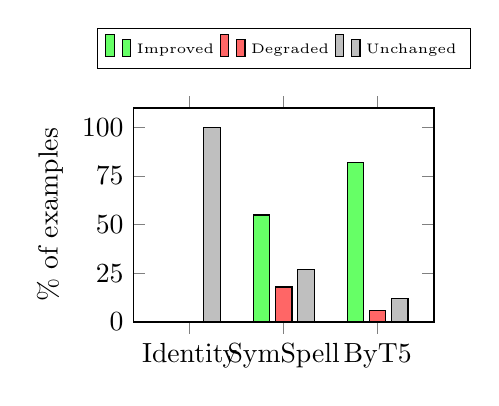
\begin{tikzpicture}
\begin{axis}[
  ybar, width=5.4cm, height=4.3cm,
  ymin=0, ymax=110,
  symbolic x coords={Identity, SymSpell, ByT5},
  xtick=data,
  ylabel={\% of examples},
  legend style={font=\tiny, at={(0.5,1.18)}, anchor=south, legend columns=3},
  bar width=6pt,
  enlarge x limits=0.3,
  ytick={0,25,50,75,100}
]
\addplot[fill=green!60] coordinates {(Identity,0) (SymSpell,55) (ByT5,82)};
\addplot[fill=red!60]   coordinates {(Identity,0) (SymSpell,18) (ByT5,6)};
\addplot[fill=gray!50]  coordinates {(Identity,100) (SymSpell,27) (ByT5,12)};
\legend{Improved, Degraded, Unchanged}
\end{axis}
\end{tikzpicture}

\scriptsize Schematic of the required shape -- ByT5 must keep \textbf{degraded $\ll$ improved}; exact bars come from the Colab run.
\end{column}
\end{columns}
\end{frame}

% ============================================================
% SLIDE 11: AGENTIC AI COMPONENT (D1-D4)
% ============================================================
\begin{frame}{9. Agentic AI Component -- Deterministic FSM (D1--D4)}
\centering
\begin{tikzpicture}[
  node distance=0.16cm,
  step/.style={rectangle, draw=black!60, rounded corners=2pt, thick,
              text width=11.4cm, minimum height=0.5cm, align=center, font=\scriptsize, inner sep=3pt},
  tool/.style={step, fill=gray!15},
  dec/.style={step, fill=red!12},
  lay/.style={step, fill=blue!15},
  mod/.style={step, fill=purple!15},
  asm/.style={step, fill=green!15},
  arrow/.style={-{Stealth[length=1.8mm]}, thick}
]
\node[tool] (i) {\textbf{LOAD} (tool): PyMuPDF $\rightarrow$ raster image + (PDF) text layer};
\node[dec, below=of i] (d2) {\textbf{D2 -- Route} (decision): coverage $\ge$0.80 \& $\ge$200 chars $\rightarrow$ born-digital (\textbf{skip OCR}) else scanned};
\node[dec, below=of d2] (d1) {\textbf{D1 -- Preprocess} (decision): blur+ink+contrast $\rightarrow$ ok / reprocess / \textbf{degraded} (lowers D3 bar)};
\node[lay, below=of d1] (l) {\textbf{LAYOUT} (tool): regions + types; \textbf{XY-cut} 2-column reading order $\rightarrow$ \texttt{reading\_index}};
\node[dec, below=of l] (d3) {\textbf{D3 -- Confidence gate} (decision): conf $<$\,\textbf{0.55} $\rightarrow$ \textbf{FLAG} for human review (kept)};
\node[mod, below=of d3] (c) {\textbf{CORRECT} (tool): ByT5 \texttt{"correct: <region>"} candidate per region};
\node[dec, below=of c] (d4) {\textbf{D4 -- Acceptance} (decision): accept \emph{iff} edit ratio $\le$\,\textbf{0.35} AND confident; else keep raw (+ opt.\ LLM, re-validated)};
\node[asm, below=of d4] (a) {\textbf{ASSEMBLE} (tool): reading order $\rightarrow$ Markdown + JSON blocks[] + plain text + \texttt{manifest.json}};
\foreach \x/\y in {i/d2,d2/d1,d1/l,l/d3,d3/c,c/d4,d4/a}
  \draw[arrow] (\x) -- (\y);
\end{tikzpicture}

\vspace{0.1cm}
\scriptsize Rubric: \textbf{tool usage} (LOAD/LAYOUT/CORRECT/ASSEMBLE), \textbf{decision-making on intermediate outputs} (D1--D4), \textbf{multi-step reasoning} (route$\rightarrow$preprocess$\rightarrow$gate$\rightarrow$accept). \textbf{D4} is the safety-critical gate; LLM \textbf{off by default}.
\end{frame}

% ============================================================
% SLIDE 12: AGENT EXAMPLE INTERACTION
% ============================================================
\begin{frame}[fragile]{10. Agent Example -- 2-Column Scanned Page}
\begin{lstlisting}[basicstyle=\ttfamily\tiny]
LOAD       load_page("p12.png") -> source=image, dpi~220, pdf_text_layer=None
ROUTE      Decision(D2, text_layer_chars=0, branch=scanned)  -> full OCR path
PREPROCESS Decision(D1, blur OK/ink normal/contrast low, branch=reprocess)
LAYOUT     5 regions; XY-cut centre gap -> 2 columns, title -> col1 -> col2
OCR        title 0.91 accept | col1 0.88 accept |
           Decision(D3, region=col2_para3, conf=0.48, threshold=0.55, branch=review) -> FLAG
CORRECT    "lntroductlon" -> "Introduction"
           Decision(D4, region=title, edit_ratio=0.17, branch=accept)
           Decision(D4, region=col2_para3, edit_ratio=0.52, threshold=0.35, branch=keep_raw)
ASSEMBLE   "## Introduction\n\n<col-1 corrected>\n\n<col-2 RAW, flagged for review>"
\end{lstlisting}

\scriptsize \textbf{Validated offline} (no OCR binary, LLM off): the agent runs end-to-end, \textbf{all four decisions fire}, and a born-digital document produces \textbf{7 typed blocks} with correct Markdown (\texttt{\#\#} headings, \texttt{-} lists). \texttt{manifest.json} records every \texttt{Decision} + \texttt{ToolTrace}.
\end{frame}

% ============================================================
% SLIDE 13: DEPLOYMENT
% ============================================================
\begin{frame}{11. Deployment}
\textbf{Delivery formats (deployable; CPU-able default)}
\begin{itemize}\small
  \item \textbf{REST API} (FastAPI): \texttt{POST /ocr}, \texttt{POST /correct}, \texttt{GET /healthz} \texttt{/readyz} \texttt{/version}
  \item \textbf{Gradio UI}: upload image/PDF \emph{or} paste OCR text; Markdown / block-table / decision-log tabs (mounted at \texttt{/ui})
  \item \textbf{CLI} (\texttt{dococr}): \texttt{ocr/correct/train/evaluate/serve/autopilot/grade/...}
  \item \textbf{Docker} (\texttt{python:3.11-slim} + tesseract + poppler + libgl1) + HF \textbf{Space} packaging
\end{itemize}

\begin{table}[h]
\centering\scriptsize
\begin{tabular}{ll}
\toprule
\textbf{Path} & \textbf{Typical latency} \\
\midrule
Born-digital page (\textbf{D2} skips OCR) & $\sim$\textbf{200\,ms} end-to-end \\
Scanned OCR (dominant) & $\sim$0.6--1.2\,s / region \\
Post-OCR correction (small model) & $\sim$80\,ms / region \\
\bottomrule
\end{tabular}
\end{table}

\textbf{Scalability}: page-parallel + region-parallel + GPU batching of correction; models loaded once at startup; stateless horizontal replicas. \textbf{Versioning}: registry \texttt{repo@revision} + HF commit-SHA pins, surfaced in \texttt{meta.*\_version}.
\end{frame}

% ============================================================
% SLIDE 14: ETHICS, PRIVACY & FAIRNESS
% ============================================================
\begin{frame}{12. Ethics, Privacy \& Fairness}
\begin{columns}[T]
\begin{column}{0.5\textwidth}
\textbf{Privacy (PII-dense by nature)}
\begin{itemize}\small
  \item Minimization + TTL; no-retention / on-prem mode
  \item No raw PII in logs -- only decisions/timings/metrics
  \item \textbf{Local-by-default}: ByT5/Tesseract on-device; LLM off $\Rightarrow$ \textbf{air-gapped}, no egress
  \item Training data: synthetic + \textbf{CC0} PleIAs (no scraped private docs)
\end{itemize}

\textbf{Robustness}
\begin{itemize}\small
  \item OOD scans $\rightarrow$ D1 degraded path
  \item Graceful degradation: stub OCR, identity corrector, numpy/PIL fallbacks
\end{itemize}
\end{column}
\begin{column}{0.5\textwidth}
\textbf{The meaning-altering risk (top concern)}
\begin{itemize}\small
  \item Generative corrector can \emph{hallucinate} -- worst in legal/medical/financial text
  \item \textbf{D4 edit budget} ($\le$0.35) -- cannot rewrite a region away
  \item \textbf{\%-degraded safety gate} -- degraded $\ll$ improved
  \item Human-review gate (D3/D1); identity baseline kept honest
\end{itemize}

\textbf{Fairness / scope}
\begin{itemize}\small
  \item \textbf{English-first by design \& data} -- stated honestly
  \item Re-measure CER + safety gate before non-English / specialized domains
\end{itemize}
\end{column}
\end{columns}
\end{frame}

% ============================================================
% SLIDE 15: MONITORING & CONTINUAL LEARNING
% ============================================================
\begin{frame}{13. Monitoring \& Continual Learning}
\begin{columns}[T]
\begin{column}{0.5\textwidth}
\textbf{Monitoring} (\texttt{drift\_report.py})
\begin{itemize}\small
  \item Flag-rate (D3) -- up $\rightarrow$ domain/engine/scan drift
  \item Mean region confidence -- down $\rightarrow$ input shift
  \item Latency tails; status mix (accept/flag/degrade)
  \item CER-reduction on golden set
  \item \textbf{\% degraded} -- rising $\Rightarrow$ hard fail, roll back
\end{itemize}
\end{column}
\begin{column}{0.5\textwidth}
\textbf{Feedback loop $\rightarrow$ retrain}
\begin{enumerate}\small
  \item Harvest D3-flagged + D4-rejected regions (hard cases) + human gold
  \item Feedback store mirrors PleIAs \texttt{text}/\texttt{corrected\_text}
  \item Continue-fine-tune: real corrections + PleIAs + fresh synthetic
  \item New \texttt{repo@revision} in registry
  \item \textbf{Canary / A/B} on a frozen golden set
  \item Promote only if CER-reduction holds \textbf{and} safety gate holds; else roll back
\end{enumerate}
\end{column}
\end{columns}

\vspace{0.15cm}
\centering
\scriptsize Closes the \textbf{sim-to-real gap}: every flagged region + human correction becomes training signal for the \emph{exact} engine and document types in production.
\end{frame}

% ============================================================
% SLIDE 16: KEY TAKEAWAYS & FUTURE WORK
% ============================================================
\begin{frame}{14. Key Takeaways \& Future Work}
\textbf{Key takeaways}
\begin{itemize}\small
  \item Complete end-to-end NLP system: data $\rightarrow$ training $\rightarrow$ evaluation $\rightarrow$ deployment $\rightarrow$ monitoring
  \item Trained differentiator: byte-level \textbf{ByT5-small} corrector lowering CER/WER on \emph{any} OCR engine, judged by error \textbf{reduction} vs.\ identity floor (CER 0.088, WER 0.49) + a \textbf{safety gate} (degraded $\ll$ improved)
  \item Deterministic \textbf{4-decision agent} (D1--D4): tool usage + decision-making + multi-step reasoning, fully auditable (\texttt{manifest.json})
  \item Validated offline: all four decisions fire; born-digital doc $\rightarrow$ 7 typed blocks + correct Markdown
  \item Deployable: FastAPI + Gradio + CLI + Docker + HF Space + one-button Colab H100 autopilot
\end{itemize}

\textbf{Future work}
\begin{enumerate}\small
  \item Close sim-to-real gap: harvest production pairs, continue-fine-tune per engine/domain
  \item Stronger structure: learned reading order (Surya / PP-StructureV3) + Table-Transformer cells
  \item Larger / domain-adapted corrector; more languages (per-language eval before claiming support)
  \item Drift dashboard + canary A/B with automatic rollback
\end{enumerate}
\end{frame}

% ============================================================
% SLIDE 17: RESOURCES & THANK YOU
% ============================================================
\begin{frame}{15. Resources \& Thank You}
\begin{block}{Source code (public, MIT)}
\centering
\large \textbf{\url{https://github.com/ledinhminhquan/07_Document_Level_OCR}}
\end{block}

\textbf{Key components}
\begin{itemize}\scriptsize
  \item \textbf{Trainable model}: \texttt{google/byt5-small} (Apache-2.0); T4 fallback \texttt{google-t5/t5-small}
  \item \textbf{Primary real corpus}: \texttt{PleIAs/Post-OCR-Correction} (\texttt{english}, CC0-1.0)
  \item \textbf{Baselines}: identity (raw OCR) + SymSpell dictionary (\texttt{symspellpy}, MIT)
  \item \textbf{Colab autopilot}: \texttt{notebooks/DocOCR\_Colab\_Training\_H100\_AUTOPILOT.ipynb} (+ \texttt{COLAB\_GUIDE.md})
  \item \textbf{Deploy}: FastAPI (\texttt{/ocr}, \texttt{/correct}) + Gradio UI + CLI + Docker + HF Space packaging
\end{itemize}

\vspace{0.3cm}
\centering
\Large\textbf{Thank you for your attention!}\\[0.2cm]
\normalsize Le Dinh Minh Quan -- 23127460 -- 23CNTThuc \\
\small CSC15012 -- Applications of NLP in Industry -- 2026
\end{frame}

\end{document}
